\documentclass{article}

% if you need to pass options to natbib, use, e.g.:
%     \PassOptionsToPackage{numbers, compress}{natbib}
% before loading neurips_2018

% ready for submission
% \usepackage{neurips_2018}

% to compile a preprint version, e.g., for submission to arXiv, add add the
% [preprint] option:
%     \usepackage[preprint]{neurips_2018}

% to compile a camera-ready version, add the [final] option, e.g.:
     \usepackage[final]{nips_2018}

% to avoid loading the natbib package, add option nonatbib:
%     \usepackage[nonatbib]{neurips_2018}

\usepackage[utf8]{inputenc} % allow utf-8 input
\usepackage[T1]{fontenc}    % use 8-bit T1 fonts
\usepackage{hyperref}       % hyperlinks
\usepackage{url}            % simple URL typesetting
\usepackage{booktabs}       % professional-quality tables
\usepackage{amsfonts}       % blackboard math symbols
\usepackage{nicefrac}       % compact symbols for 1/2, etc.
\usepackage{microtype}      % microtypography
\usepackage{graphicx}
\usepackage{subcaption}

\graphicspath{ {imgs/} }

\title{CS 7180 Milestone 1}

% The \author macro works with any number of authors. There are two commands
% used to separate the names and addresses of multiple authors: \And and \AND.
%
% Using \And between authors leaves it to LaTeX to determine where to break the
% lines. Using \AND forces a line break at that point. So, if LaTeX puts 3 of 4
% authors names on the first line, and the last on the second line, try using
% \AND instead of \And before the third author name.

\author{%
  Nalin Gupta \\
  \texttt{gupta.nal@husky.neu.edu} \\
  \And
  Christopher Botica\\
  \texttt{botica.c@husky.neu.edu} \\
  \And
  Tyler Brown\\
  \texttt{brown.tyler@husky.neu.edu} \\
  % Coauthor \\
  % Affiliation \\
  % Address \\
  % \texttt{email} \\
  % \AND
  % Coauthor \\
  % Affiliation \\
  % Address \\
  % \texttt{email} \\
  % \And
  % Coauthor \\
  % Affiliation \\
  % Address \\
  % \texttt{email} \\
  % \And
  % Coauthor \\
  % Affiliation \\
  % Address \\
  % \texttt{email} \\
}

\begin{document}
% \nipsfinalcopy is no longer used

\maketitle

\section{Replication}

Using the GitHub repository provided by Chen et. al. \cite{chen2018learning},
we were able to run their code but ran into limitations with computational
resources. Chen et. al. \cite{chen2018learning} used a separate model for
each of the two cameras. They specified a minimum of 64GB of GPU RAM for the
Sony model and 128 GB of GPU RAM for the Fuji model. We decided to try
replicating the less resource intensive Sony model.

\subsection{Computing Training Parameters}

The hardware requirements for this model are nontrivial so we have explored
several options.

\begin{enumerate}
\item Using AWSEducate did not work
  \begin{itemize}
    \item Unable to create roles with IAM authentication so it's really
	 hard or impossible to move data from a S3 Bucket to an EC2 Instance
    \item Tried to create a $p3.8xlarge$ instance but these instances are
      not allowed even though they are listed
  \end{itemize}
\item Using regular AWS does work but is costly
  \begin{itemize}
    \item Ran a single AWS EC2 $p3.8xlarge$ instance with 32 CPU, 244 GB of
	 Memory, 4 Tesla V100 GPUs, and 64 GPU Memory. This costs \$12.24
	 an hour.
    \item This is the amount of GPU Memory requested by the paper
      authors as a minimum amount
    \end{itemize}
\end{enumerate}

Given these initial facts, we then tried to estimate run time requirements
for the Sony model. We trained the Sony model for 90 minutes using an
AWS $p3.8xlarge$ instance. We were able to complete $\approx 12$ training
epochs. We then tried to use the training parameters to
test the model but could not get this to work without modifying the script
provided by Chen et. al. \cite{chen2018learning}. The model parameters
were available to download, we used these parameters to run against test
data for 30 minutes. Additional time was required to extract the Sony dataset
which decompressed to about 115GB of image files. We estimate that
replicating the Chen et. al. \cite{chen2018learning} training parameters
for \textit{only} the Sony model takes approximately 500 hours or
\$ 6,120.

\subsection{Test Results from SID Model Parameters}

Figure \ref{train} contains example training data. Figure \ref{test}
contains example test results. Both Figure \ref{train} and Figure \ref{test}
are pictures of a similar yellow bike. We can see a qualitative improvement
across the three renderings of the same predicted test image in
Figure \ref{test}.

\section{Appendix}

\begin{figure}[h!]
  \centering
  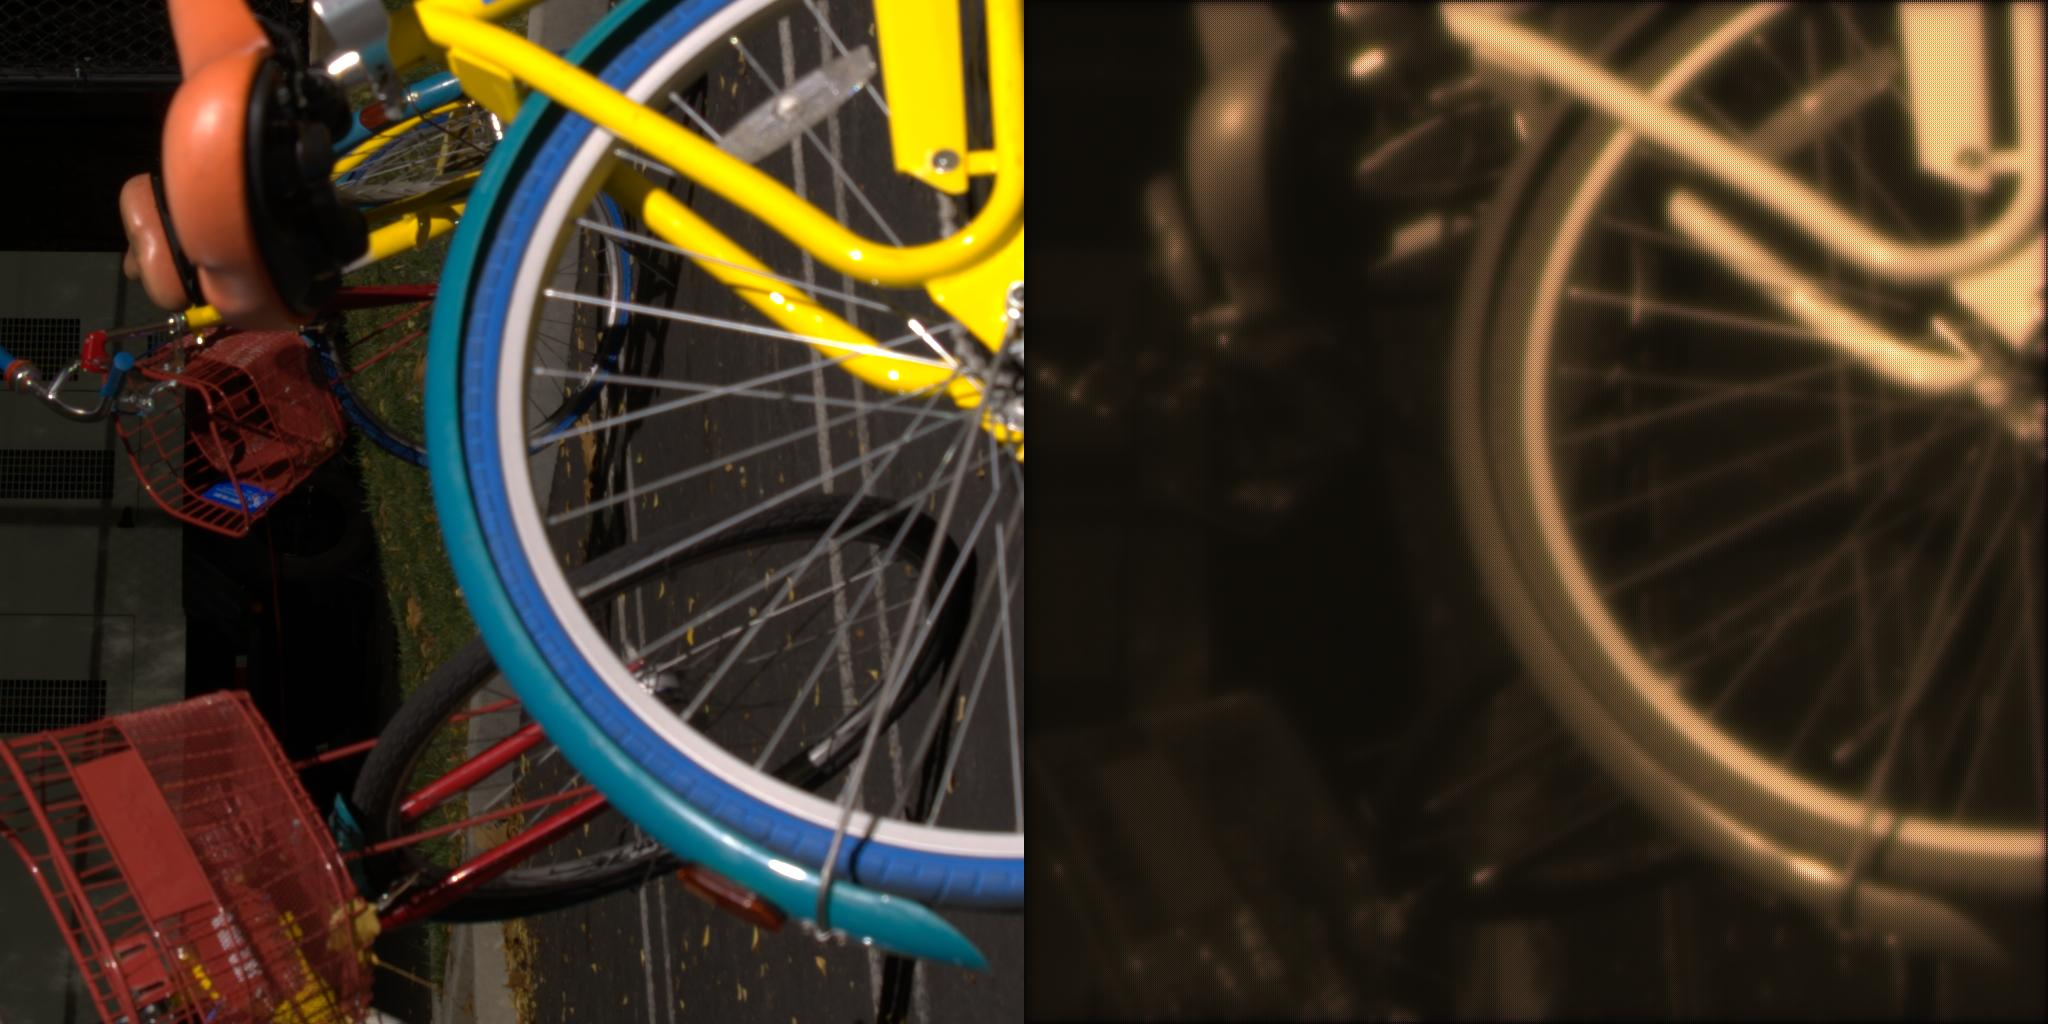
\includegraphics[scale=0.1]{00002_00_train_100}
  \caption{\label{train} Example Training Data}
\end{figure}



\begin{figure}[h!]
  \centering
  \begin{subfigure}[b]{0.3\textwidth}
    \includegraphics[width=\textwidth]{10016_00_100_gt}
    \caption{gt}
  \end{subfigure}
  \begin{subfigure}[b]{0.3\textwidth}
    \includegraphics[width=\textwidth]{10016_00_100_out}
    \caption{out}
  \end{subfigure}
  \begin{subfigure}[b]{0.3\textwidth}
    \includegraphics[width=\textwidth]{10016_00_100_scale}
    \caption{scale}
  \end{subfigure}
  \caption{\label{test} Example Test Data}
\end{figure}

\bibliographystyle{unsrt}
\bibliography{references}

\end{document}
